\chapter{$A_0$, $A_{UU}^{\cos\phi_h}$, and $A_{UU}^{\cos 2\phi_h}$}
\label{cha:A0AcAcc}

After events have been selected and binned, and after all corrections have been applied, the $\phi_h$ distributions for each $x-Q^2-z-P_{h\perp}^2$ bin are fit with the function $a(1 + b\cos\phi_h + c\cos 2\phi_h)$.
The parameters $a$, $b$, and $c$ then directly give $A_0$, $A_{UU}^{\cos\phi_h}$, and $A_{UU}^{\cos 2\phi_h}$ for each $x-Q^2-z-P_{h\perp}^2$ bin.
A complete table of results can be found in the ancillary files.
Several representitive plots are shown here in figure~\ref{fig:A0AcAcc_zPT2bins_x1QQ1_final}, which shows $A_0$, $A_{UU}^{\cos\phi_h}$, and $A_{UU}^{\cos 2\phi_h}$ vs $P_{h\perp}^2$ for several $z$ bins for both pion channels.
Several of the fits used to obtain figure~\ref{fig:A0AcAcc_zPT2bins_x1QQ1_final} are shown in figure~\ref{fig:phihFits_PT2bins_x1QQ1z6_final}.
%
\begin{figure}[htp]
\centering
\vspace{-1.5cm}
\makebox[\textwidth][c]{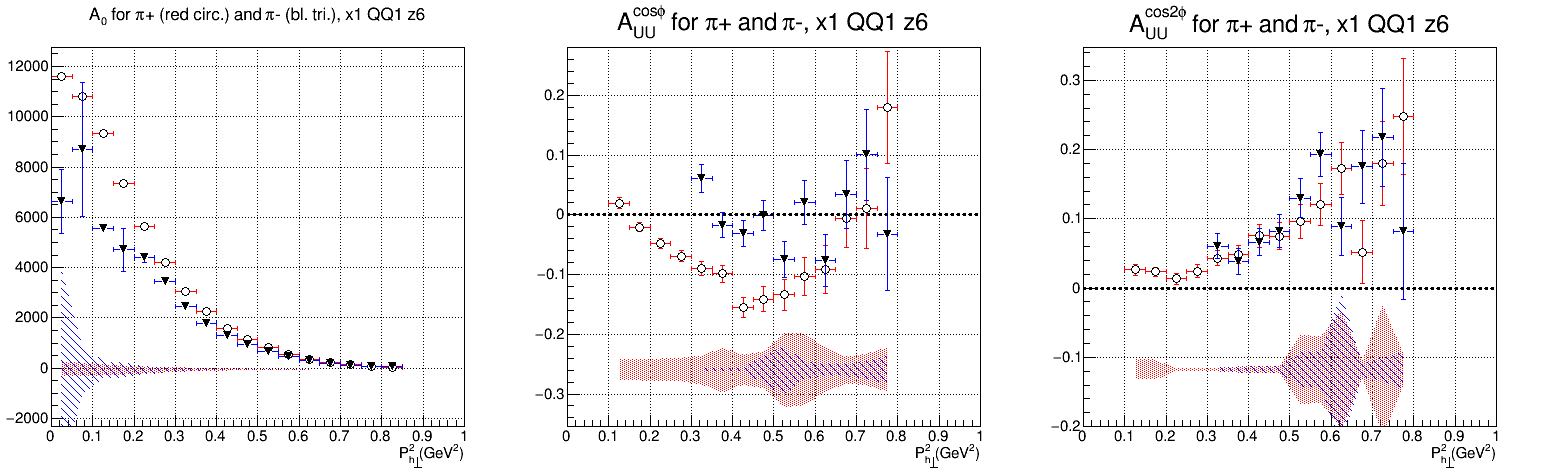
\includegraphics[width=6.5in]{figures/A0AcAccVPT2_x1QQ1z6.png}} % this centers it more nicely
\makebox[\textwidth][c]{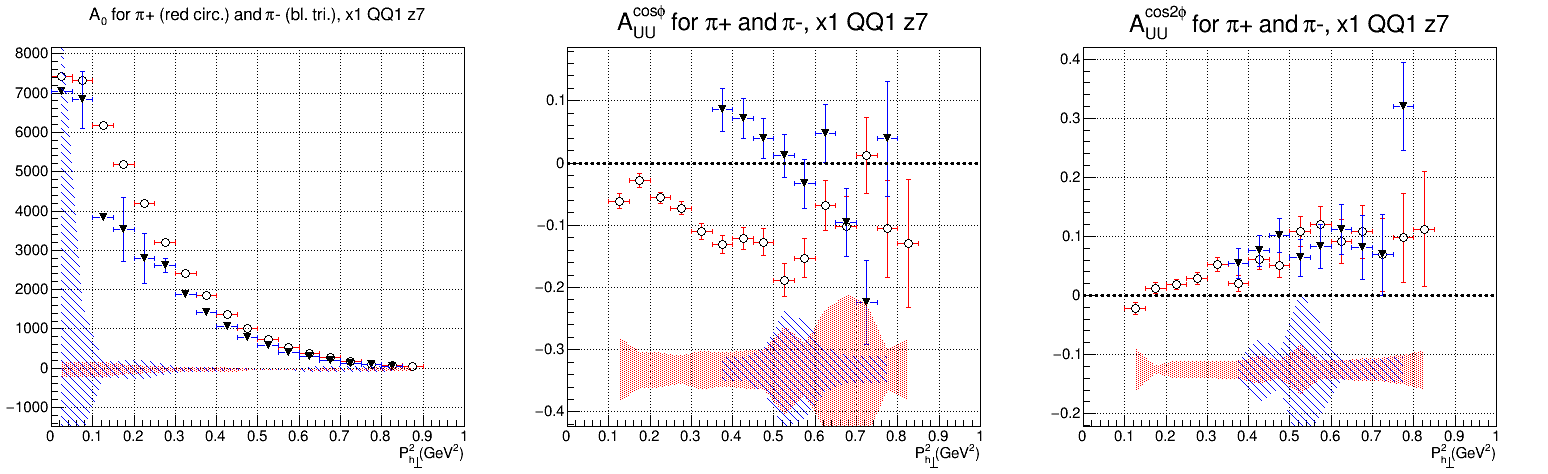
\includegraphics[width=6.5in]{figures/A0AcAccVPT2_x1QQ1z7.png}} % this centers it more nicely
\makebox[\textwidth][c]{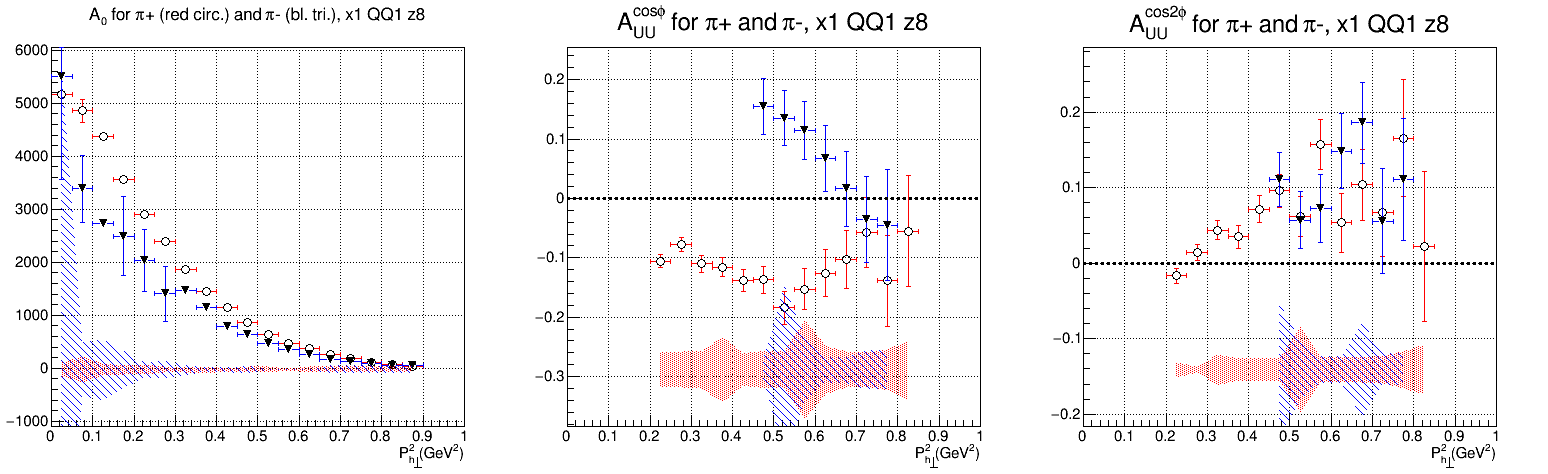
\includegraphics[width=6.5in]{figures/A0AcAccVPT2_x1QQ1z8.png}} % this centers it more nicely
\makebox[\textwidth][c]{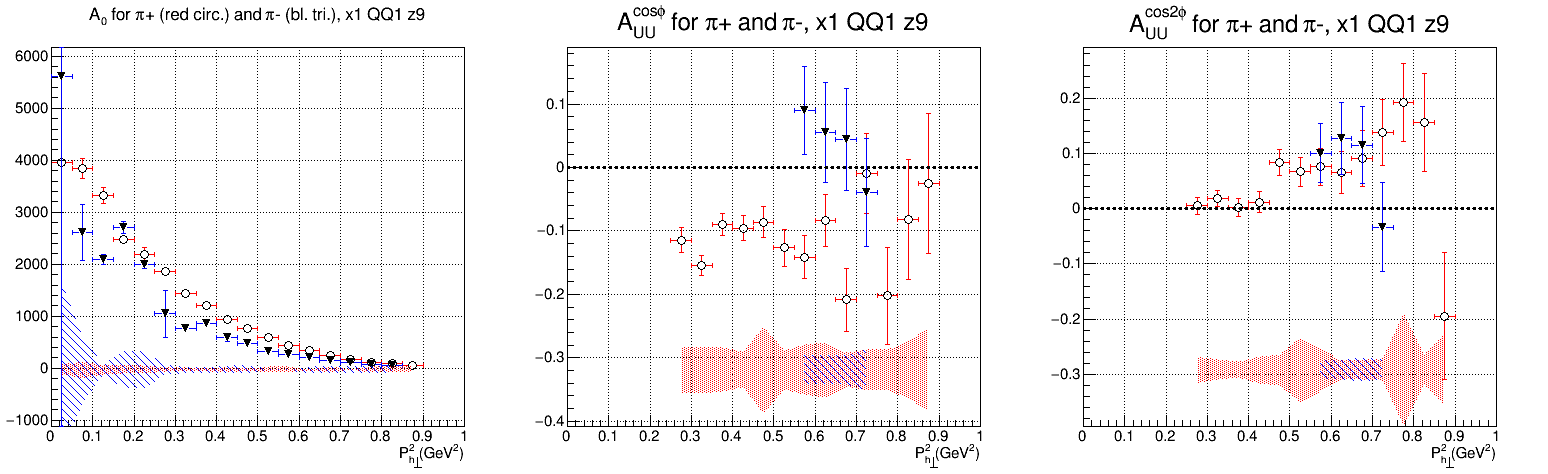
\includegraphics[width=6.5in]{figures/A0AcAccVPT2_x1QQ1z9.png}} % this centers it more nicely
\caption{$A_0$ (left column), $A_{UU}^{\cos\phi_h}$ (middle column), and $A_{UU}^{\cos 2\phi_h}$ (right column) vs $P_{h\perp}^2$ for $\pi+$ (red circles) and $\pi-$ (blue triangles). The $x$-$Q^2$ bin is fixed (the high $Q^2$ of $0.2 < x < 0.3$). Several $z$ bins are shown: $0.30 < z < 0.35$ (top row), $0.35 < z < 0.40$ (second row), $0.40 < z < 0.45$ (third row), $0.45 < z < 0.50$ (bottom row).}
\label{fig:A0AcAcc_zPT2bins_x1QQ1_final}
\end{figure}
%
\begin{figure}[htp]
\centering
\vspace{-1.5cm}
\makebox[\textwidth][c]{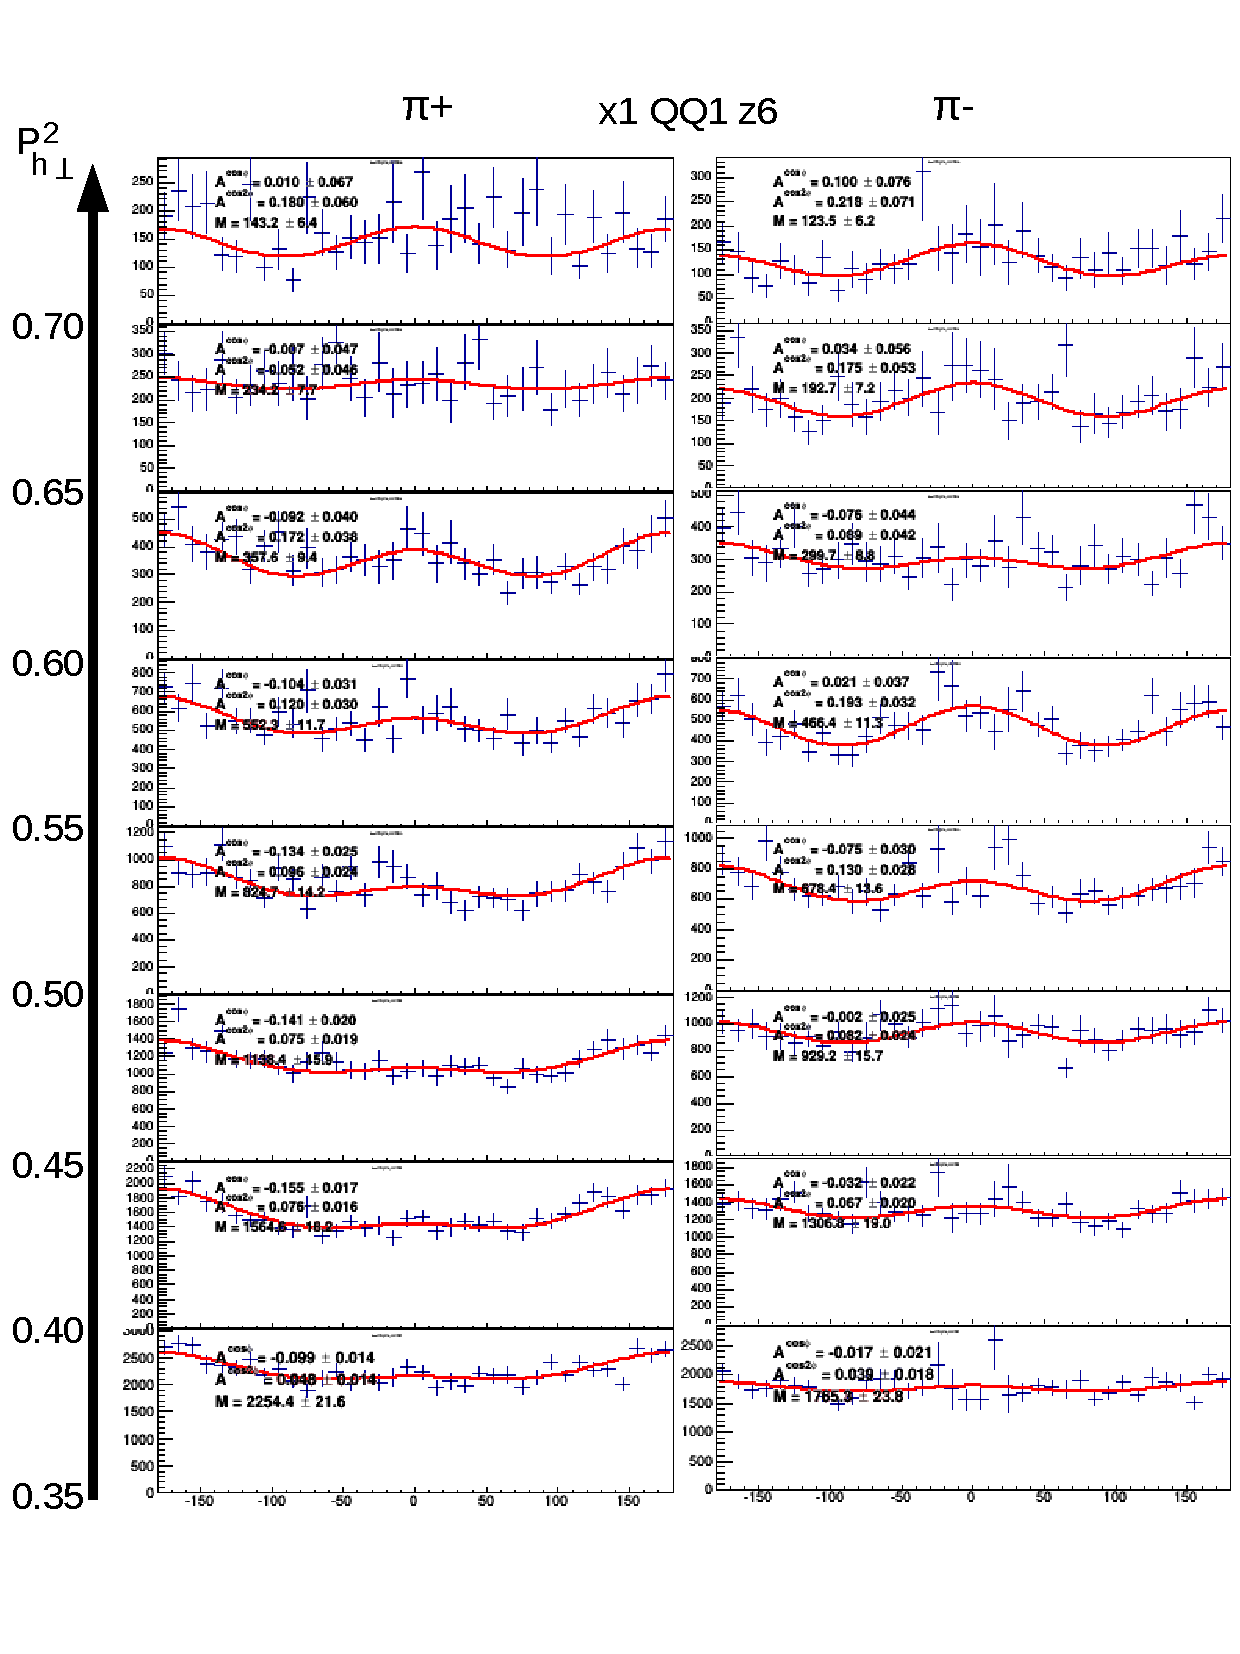
\includegraphics[width=6.5in]{figures/phihFits_PT2bins_x1QQ1z6_final.pdf}} % this centers it more nicely
\caption{Fits of several of the $\phi_h$ distrubutions used to obtain figure~\ref{fig:A0AcAcc_zPT2bins_x1QQ1_final}. The rows are bins of $P_{h\perp}^2$ as shown by the large axis on left. $\pi^+$ results are shown in the left column and $\pi^-$ on the right. These results are from the high $Q^2$ bin of $0.2 < x < 0.3$ and $0.3 < z < 0.35$.}
\label{fig:phihFits_PT2bins_x1QQ1z6_final}
\end{figure}
%
\clearpage
